\subsection{Chainer-MNIST}
%
The intention of this section is to evaluate the performance of a handwritten digit recognition application that uses pyMIC2 to perform parts of computation on Intel Xeon Phi coprocessor. Our experimental evaluation focuses on two aspects. The first one is the different between CPU and coprocessor computing capabilities, the other one is the potential of using pyMIC2 in deep learning applications.
\subsubsection{Chainer-numpy:}
%
Chainer is a well-known framework for Artificial Neural Network(ANN). One of its advantages is flexibility, which enables its users to create complex architectures simply and intuitively. Similar to TensorFlow, Caffe or Theano, Chainer uses backpropagation algorithm \cite{backprop} for training data and adjusting network's parameters. However, by using "Define-by-Run" scheme,  the network is defined on-the-fly while running actual forward computation, it makes an network created by Chainer become easier to debug than other frameworks. Therefore, an application written by Chainer integrated pyMIC2 has a faster development time.
%

\subsubsection{Experimental Setup:}
%

Our experiments are performed on a combination of CPU Intel Xeon E5 and Intel Xeon Phi 7120P coprocessor. The technical specifications of our system are described in Table \ref{tab:sys-spec} . The framework is compiled for coprocessor using Intel compiler version 17.0.4 as well as OpenMP parallel programming API implementation by Intel  and MKL [*]version. All measurements are carried out 100 times and averaged to eliminate variances in the resulting measurements.
%
\begin{table}[]
\centering
\caption{Hardware specifications}
\label{tab:sys-spec}
\begin{tabular}{|c|c|c|}
\hline
\textbf{Codename} 	& \textbf{CPU} 	& \textbf{Coprocessor} \\ \hline
\textbf{Model} & Intel Xeon E5-2680V3  & Intel Xeon Phi 7120P \\
\textbf{Microarchitecture} & Sandy Bridge EP & Intel Many Integrated Core \\
\textbf{Clock frequency} & 2.50/3.30 GHz & 1.24/1.33 GHz \\
\textbf{Memory Size} & 512 GB & 16 GB \\
\textbf{Cache} & 30.0 MB SmartCache & 30.5 MB L2 \\
\textbf{Max Memory Bandwidth} & 68 GB/s & 352 GB/s\\
\textbf{Core/Threads} & 12/24 & 61/244 \\
\hline
\end{tabular} 
\end{table}


We evaluate our approach using the MNIST \cite{mnist} dataset of handwritten digits including training set of 60,000 examples,  and 10,000 test images, each image contains 28x28 pixel grey levels. The architecture of testing ANNs has 1000, 1500, 2000, 2500 ... 5500 units, each unit represents a node in the network's hidden layer. In order to simplify the performance evaluation process, we just modify the ANNs with one hidden layer, which means our ANNs have only 3 layers which are input, output and hidden. Detailed information of the ANNs used in our evaluation are shown in Table \ref{tab:ann-info}.
%
\begin{table}[]
\centering
\caption{ANN architecture}
\label{tab:ann-info}
\begin{tabular}{|c|c|}
\hline
\multicolumn{2}{|c|}{\textbf{ANN Configuration}}\\ \hline
\textbf{Layer} 	& 3 \\
\textbf{Batch Size} & 60000 \\
\textbf{Connetion Function} & Linear  \\
\textbf{Activation Function} & Relu  \\
\textbf{Loss Function} & Softmax Cross Entropy \\
\textbf{Gradient Method} &  Stochastic gradient descent \\
\hline
\end{tabular} 
\end{table}
\subsubsection{Result:}
%
We perform entire evaluation on Docker \cite{docker} in order to easily customize the constraints of system resources. A simple experiment is conducted to ensure that the execution of the ANNs in Docker is similar to physical machine and we obtain the expected result. Thereafter, we start to evaluate the performance of applications, written by two versions of Chainer, one is original version and the other is pyMIC2 integrated version, called Chainer-XP, to execute on Intel Xeon Phi coprocessor.

\begin{figure}[]
\centering

\includegraphics[scale=0.6]{img/a.pdf}
\caption{Chainer-XP sigle core and full core}
\label{fig:1-core-and-full-core}
\end{figure}

Results presented for Chainer-XP in Figure \ref{fig:1-core-and-full-core} show that all experiments of our ANNs training corresponding to the number of units: 1000, 2000, 3000, 4000 and 5000, are executed in roughly equal time periods without being influenced by the number of CPU cores. That also means most of the computational functions have been offloaded into Intel Xeon Phi coprocessor. Moreover, it can be seen that the data communication occupies most of the execution time of training process, overhead is caused by the synchronization between CPU(host) and coprocessor(device) during the calculation. Overall, pyMIC2 is a potential framework which supports its users run ANNs entirely on Intel Xeon Phi. However, the synchronization occupies a prominent role throughout the training process, if it is not tightly controlled, the performance can be devastatingly reduced.


In this experiment, we evaluate pyMIC2's computational capabilities in Intel Xeon Phi. The first ANN (ANN-1) written by original Chainer is executed on a Docker that used full core of a CPU Intel Xeon E5, and the other ANN(ANN-2) written by Chainer-XP on a Docker used only one core combined with Intel Xeon Phi coprocessor. In detail, both ANNs contain three layers and 1000 units in hidden layer, the network's configuration details are described in the Table \ref{tab:ann-info}. Then we measure thoroughly the computation time of all functions during training process and find out that with the second ANN calculation time on coprocessor occupies just approximately 29.2\% total run time. More specifically, with a mentioned ANN, the calculation is mainly executed in \textit{dot} function, about 90.2\% of computation time as it is called three times each training.
\begin{figure}[]
\centering
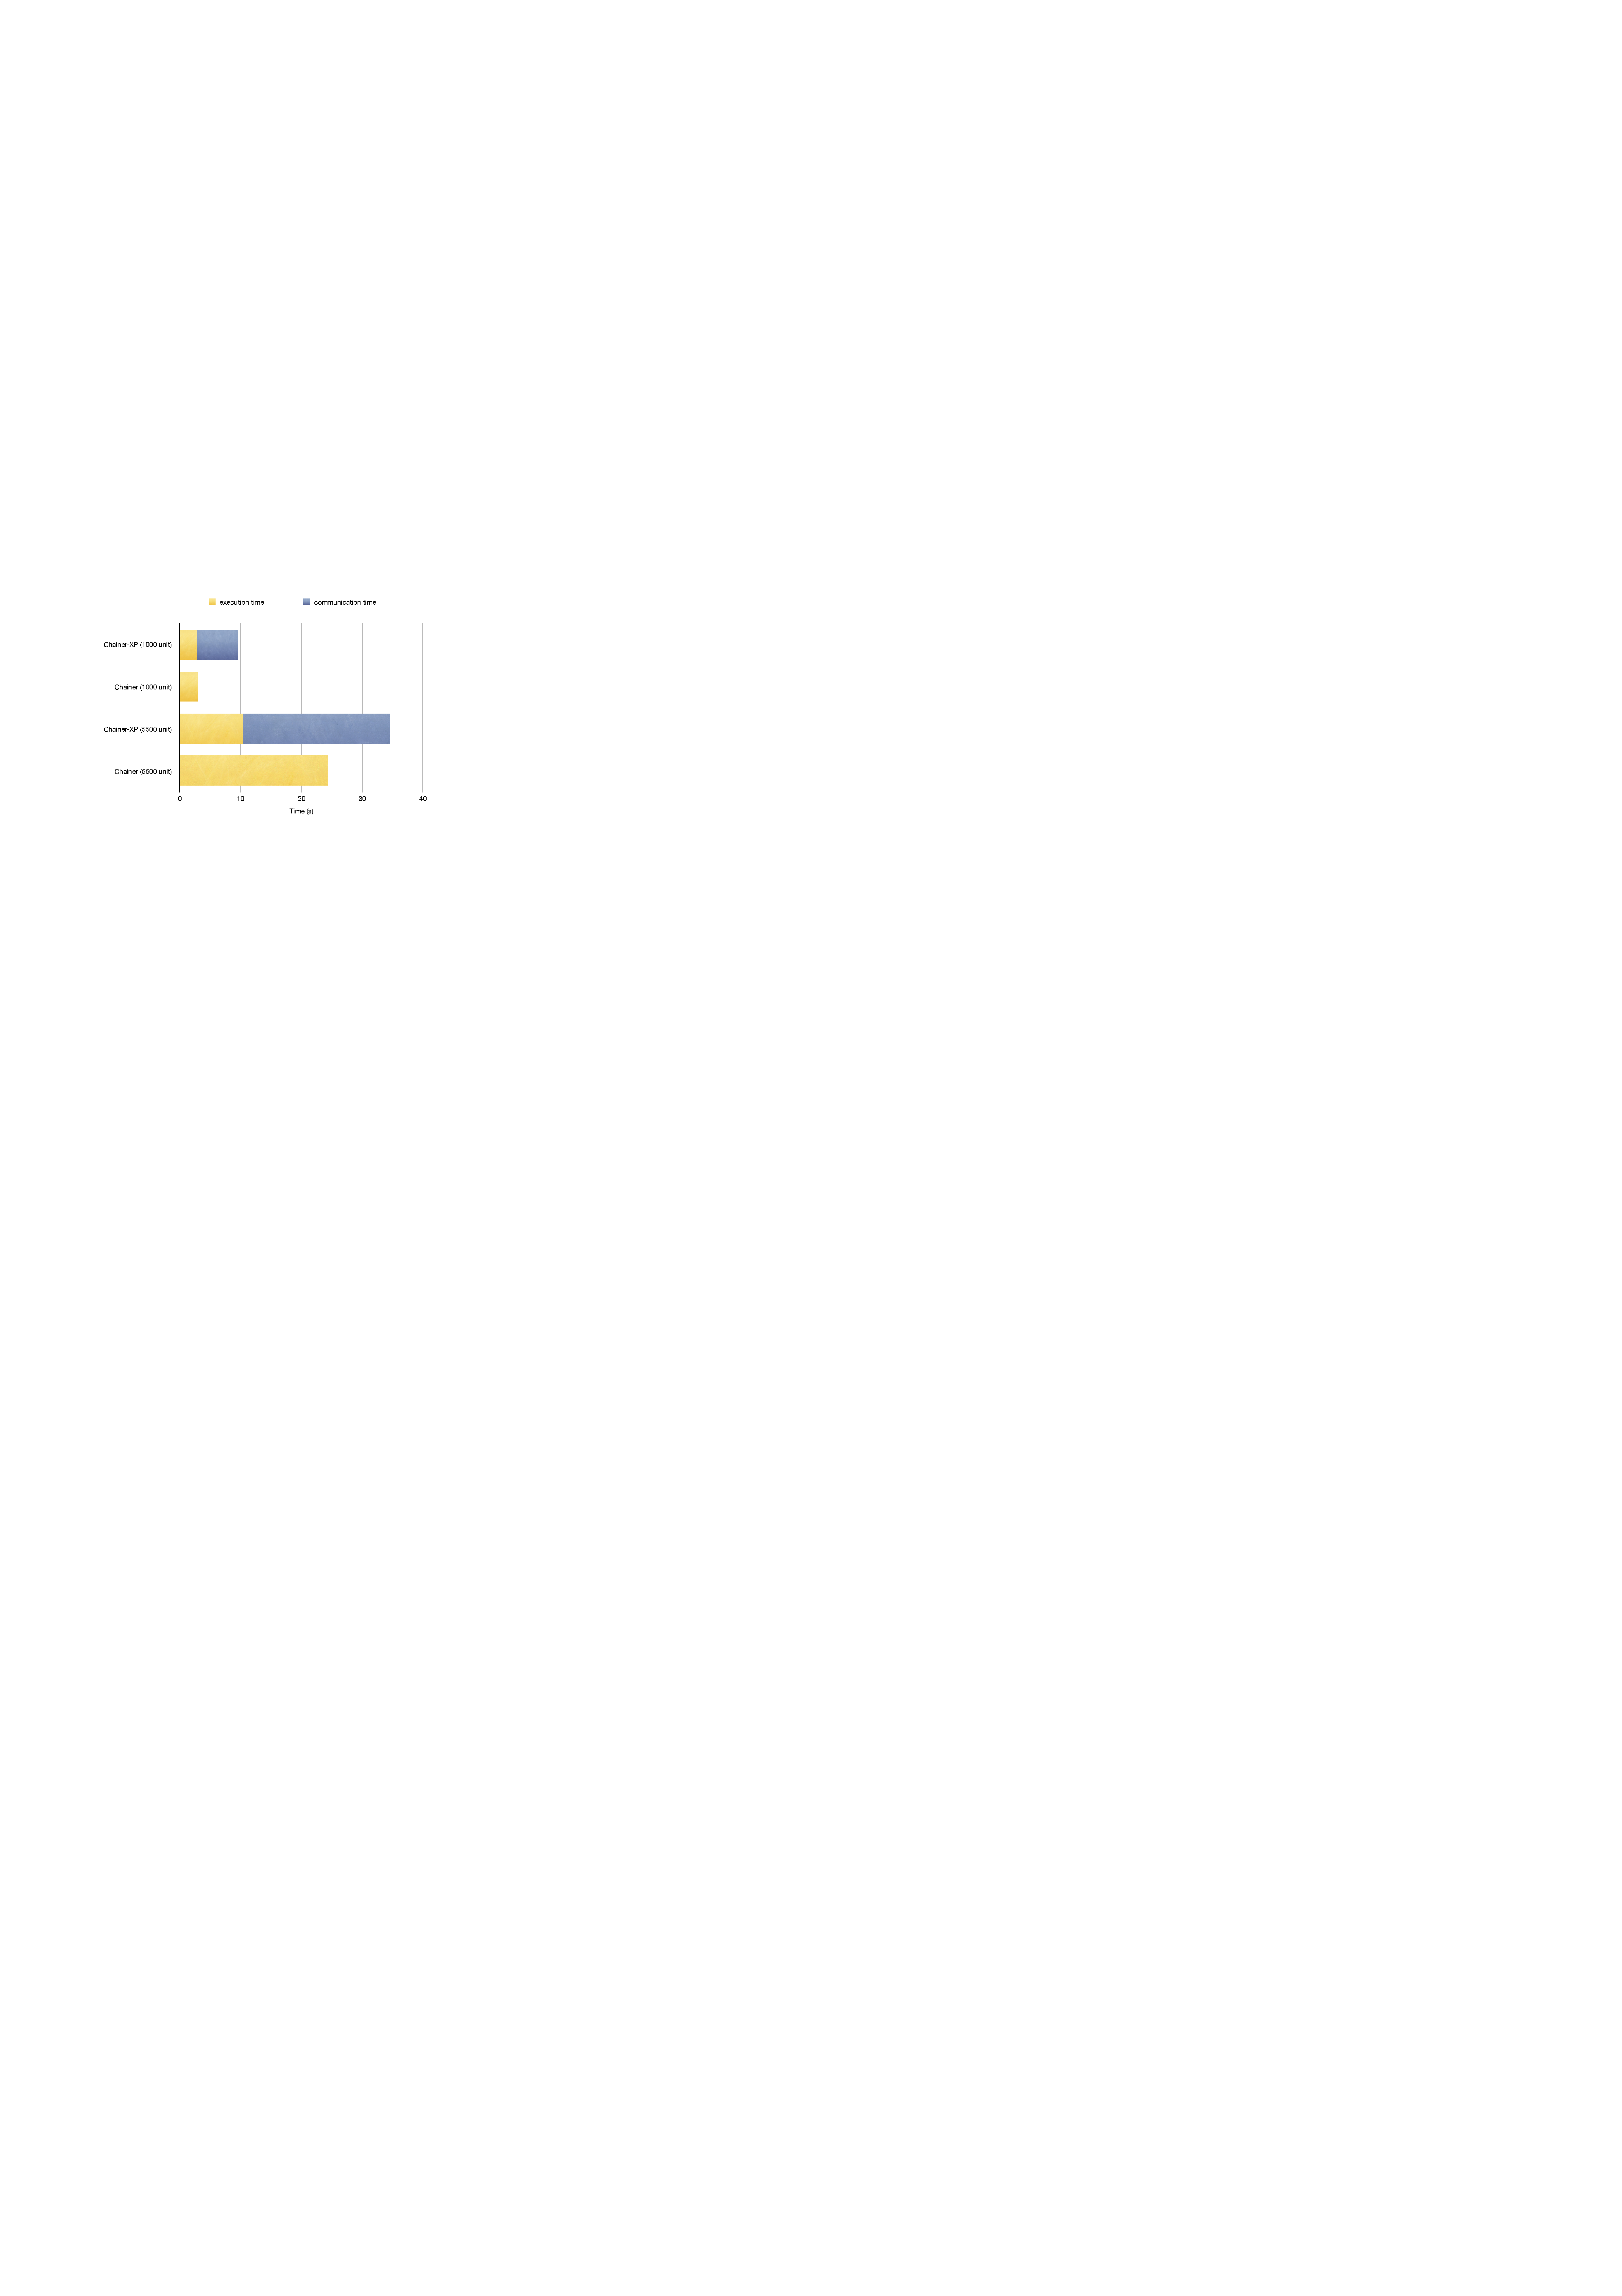
\includegraphics[scale=0.5]{img/b.pdf}
\caption{Chainer-XP single core and 12 core}
\label{b.pdf}
\end{figure}

The biggest matrix size that the \textit{dot} function must perform during the execution of the above network is [784,60000] x [60000,1000], which corresponds to 70.8\% total run time used to synchronize data between host and device. Although the purely computation time of ANN-2 on the coprocessor is approximately 1.93 times faster, the total training time was about 1.78 times slower than ANN-1 on the full core CPU. The reason for this drop in performance is transmitting data between hosts and devices repeatedly leading to overlap and redundancy. However, the cause of this result is that the pyMIC2 integration into Chainer has not been optimized, therefore, we can significantly improve the result as pyMIC2 provides objects and functions that strictly support memory allocation and deallocation on Intel Xeon Phi coprocessor. In other words, we must fully understand how Chainer organizes the data so that we can reduce the communication between host and device and increase the performance of training process. As mentioned above, in this paper we just focus on the computing capabilities; thus, in the rest of the experiment, the number of units is raised to 5500 with the aim of increasing the size of the largest matrix to [784,60000] x [60000,5500]. The observed result shows that the ratio between computation time on coprocessor and total training time is almost unchanged at about 30\%. In addition, when the size of one of the two \textit{dot} operands expanded 5.5 times, the computation time on the Intel Xeon Phi increased only 3.8 times, while the CPU run time is grown up to 7.8 times, and total training time achieve 1.2 times faster than CPU. Thus, with several medium configuration CPUs, there is the possibility that we can speed up with Intel Xeon Phi for large-scale computing in ANNs.
\begin{figure}[]
\centering
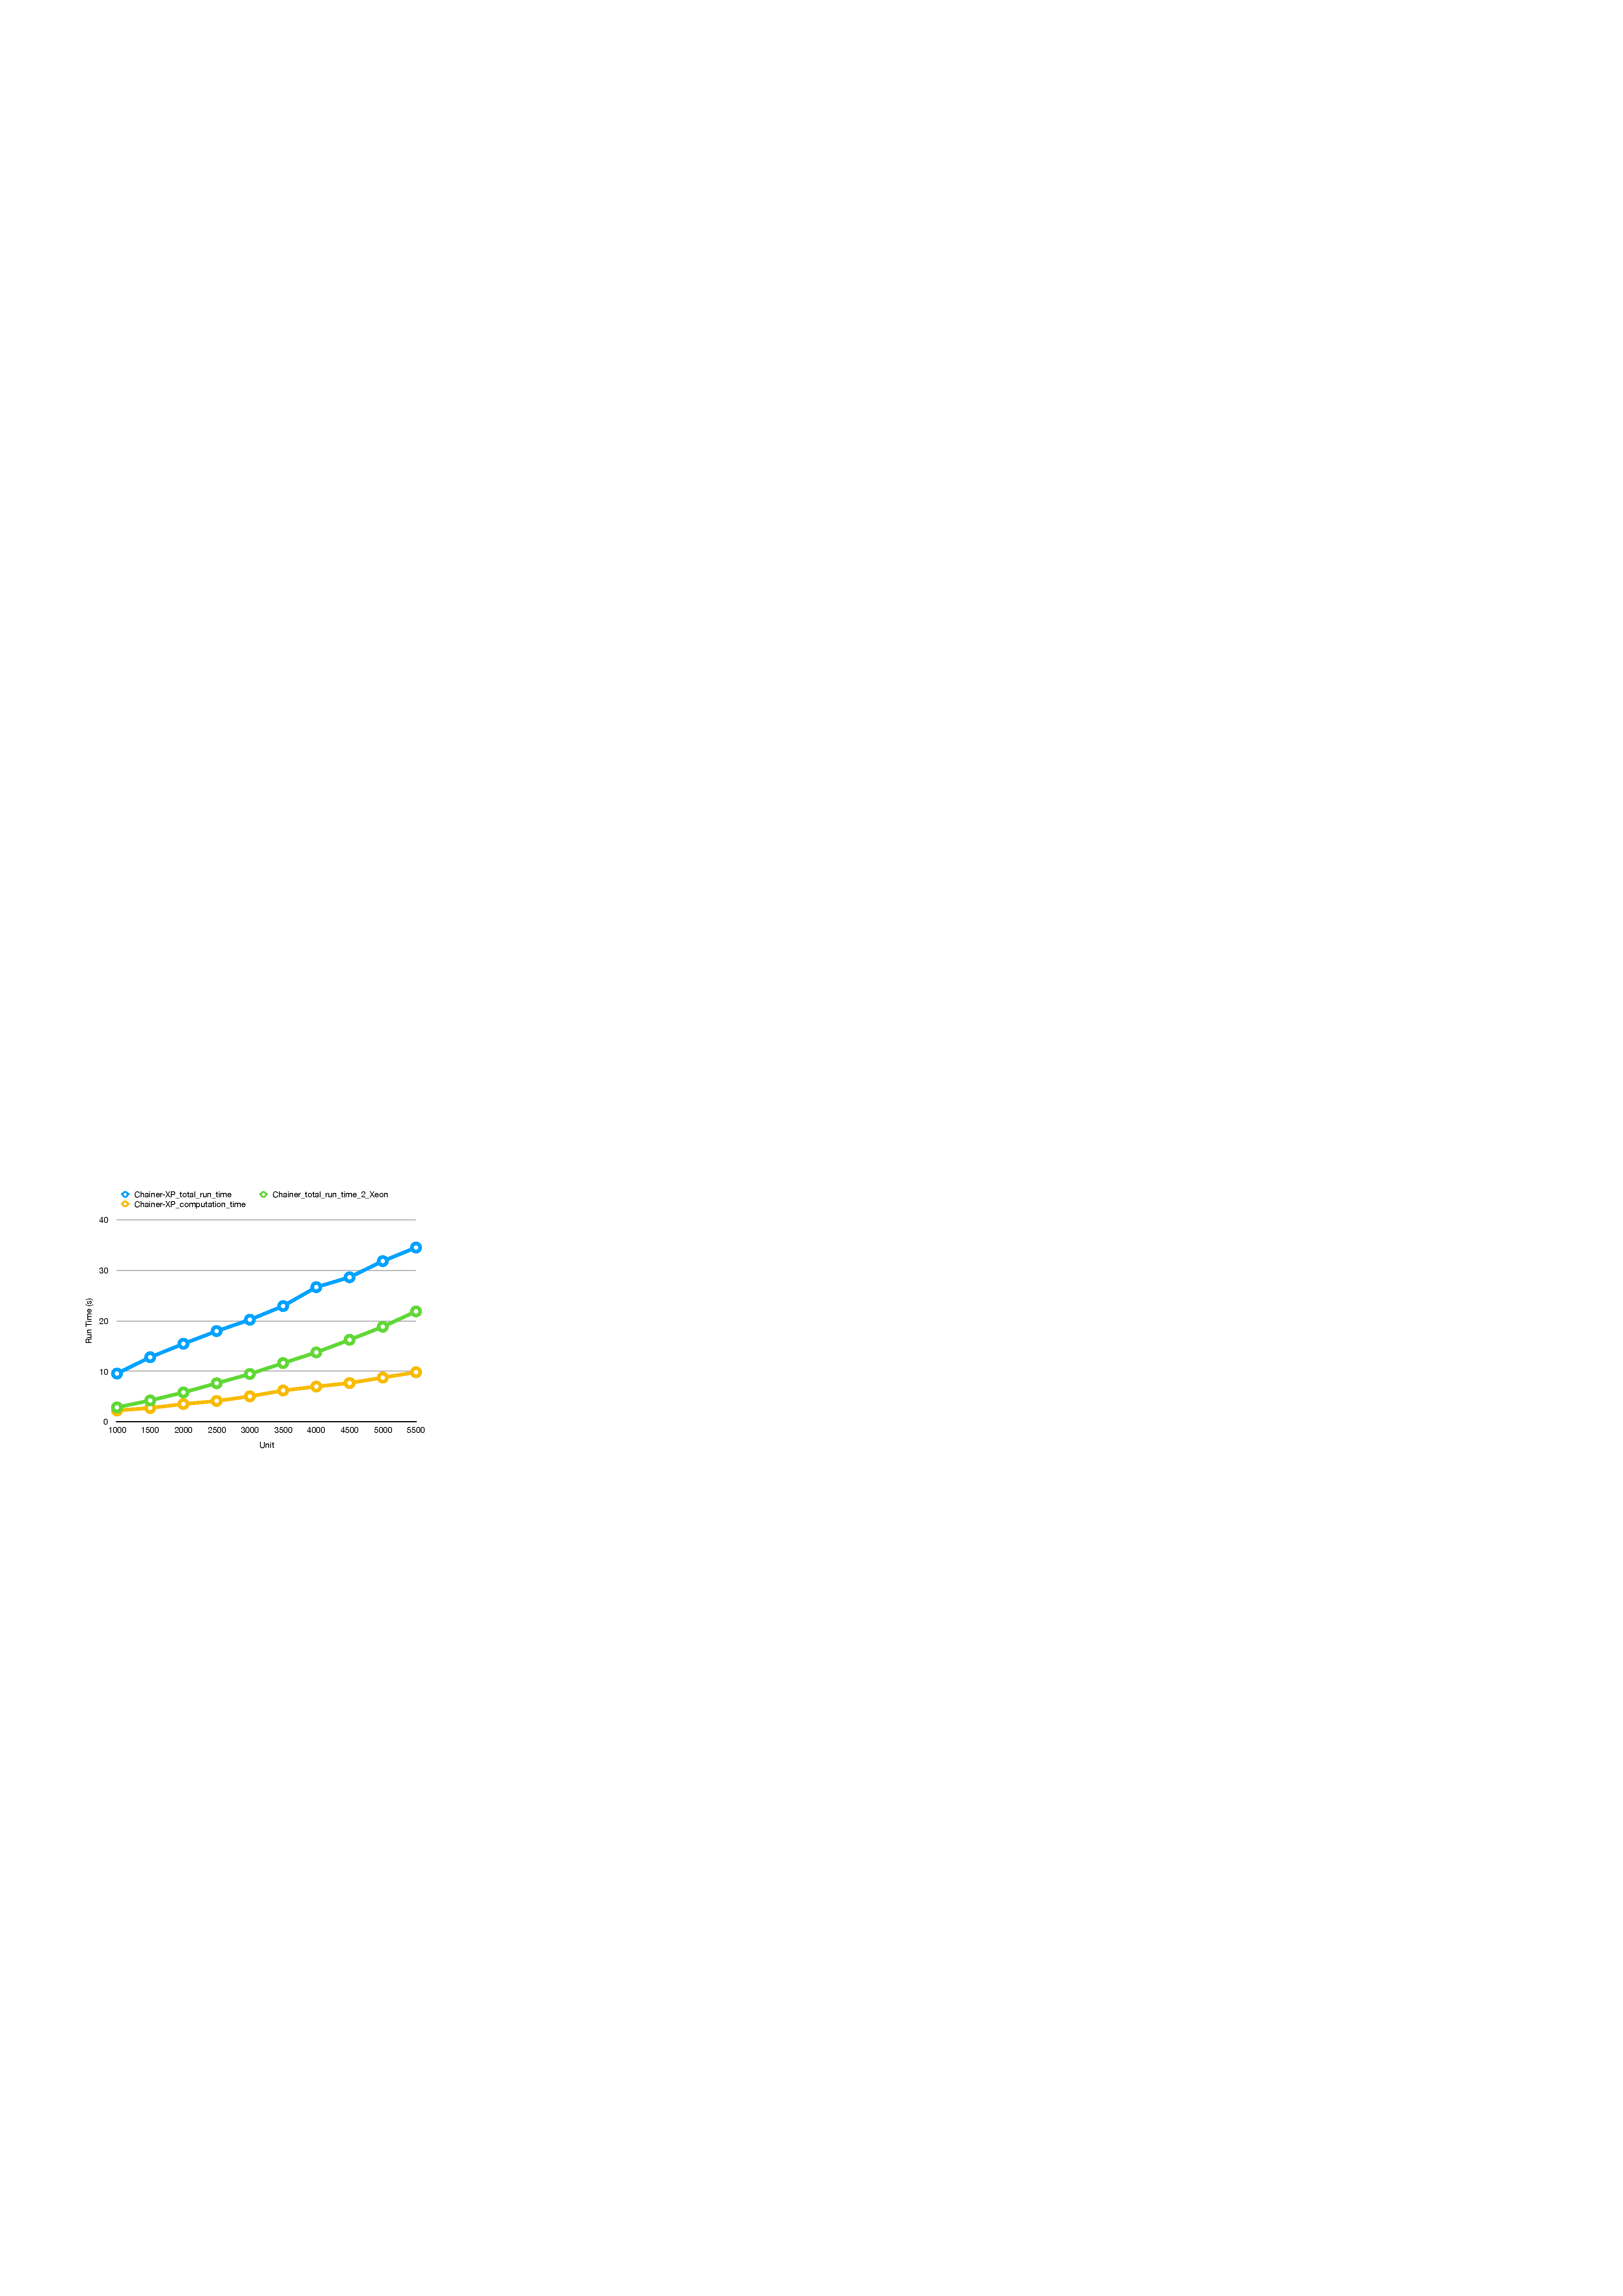
\includegraphics[scale=0.6]{img/c.pdf}
\caption{Chainer-XP vs Chainer}
\label{chainer-xp-vs-chainer}
\end{figure}

The comparison between two versions of Chainer is illustrated in Figure \ref{chainer-xp-vs-chainer}. In order to obtain this experience, The ANN-1 is executed entirely on CPU with a Docker containing dual-processor Intel Xeon E5, which has computing capability approximately 960 GFLOP/s, while the peak performance of an Xeon Phi coprocessor is approximate 1 TFLOP/s \ref{halyo2014first} in double precision. Although they almost have the similar processing power, computation time of an ANN integrated pyMIC2  is getting faster and faster than this ANN which runs in CPU. Hence, It can be seen that pyMIC2 has used the Xeon Phi's SIMD mechanism, as well as Vectorization technique of Intel Xeon Phi quite effectively in calculating sequential elements.
